\section{Large worlds of mathematical structures}
\subsection{Monoids and Homomorphisms}
Suppose some function $f: \mathbb{N} \rightarrow \mathbb{Z}$ and $f(n)=n$. This function
$f$ respects addition in the following sense.
\begin{align*}
    f(m+n) = f(m) + f(n)
\end{align*}
We can add $m+n$ first and then map it via $f$, or we can first map $m, n$ via
$f$, and then add them.

\begin{ttta}
Another possible function $f: \mathbb{N} \rightarrow \mathbb{Z}$ is given by
$f(n) = 2n$. See if you can check that this also satisfies the above condition
$f(m+n) = f(m) + f(n)$.
\begin{align*}
    f(m+n) =& f(m) + f(n)\\
    2(m+n) =& 2(m) + 2(n)\\
    2(m+n) =& 2(m+n)\\
    m+n =& m+n
\end{align*}
Thus we have shown that $f$ respects addition.
\end{ttta}

\begin{ttta}
Show that this function
\[
f=\set{(0, 0), (1, 1), (2, -1), (3, 2), (4, -2), (5, 3), (6, -3), \dots}
\]
does not respect addition.
\begin{align*}
    f(1+3) =& f(1) + f(3)\\
    f(4) =& f(1) + f(3)\\
    -2 =& 1 + 2\\
    -2 \neq& 3
\end{align*}
\end{ttta}

\begin{ttta}
Mapping into the integers is special because it turns out that respecting
addition forces a function to respect the identity. Prove it.
\end{ttta}
\begin{proofitem}
\item To respect addition a function $f$ must satisfy the following equation $f(m+n) =
f(m)+f(n)$.  Let us suppose that $f$ does respect addition and show that it
implies that $f$ also respects the identity.
\begin{align*}
    f(0+n) =& f(0) + f(n)\\
    f(n) =& f(0) + f(n)\\
    f(0) =& 0
\end{align*}
\end{proofitem}
\begin{definition}
Let $A$ and $B$ be monoids, and write the identity as $1$ and the
binary operation as $\circ$ in each case. Then a monoid homomorphism from A to
B is a function $f:A\rightarrow B$ on the underlying sets, such that
\begin{align*}
    \forall x, y \in A, f(x \circ y) &= f(x) \circ f(y)&&f\text{ respects }\circ\\
    f(1)&=1&&f\text{ respects identity}
\end{align*}
\end{definition}

\begin{ttta}
What do we need to check to show that monoids and their homomorphisms form a
category?
\end{ttta}
\begin{proofitem}
\item Let $M$ be the set of monoids, where each element is a monoid.
\item Let $\mathcal{C}_\text{mon}$ be a category where each object is a monoid
    $A\in M$, and each arrow $\times$ is a mapping $A,B \in M, \times:
    A\rightarrow B$.
\item Let $\circ$ be the monoidal operation of an object
    $A\in\mathcal{C}_\text{mon}$, and let $\times$
    be the mapping between objects of the category $\mathcal{C}_\text{mon}$.
\item To show that monoids and their homomorphisms form a cateogry we must show
    the properties of unitality and associativity.
\begin{figure}
   \centering
   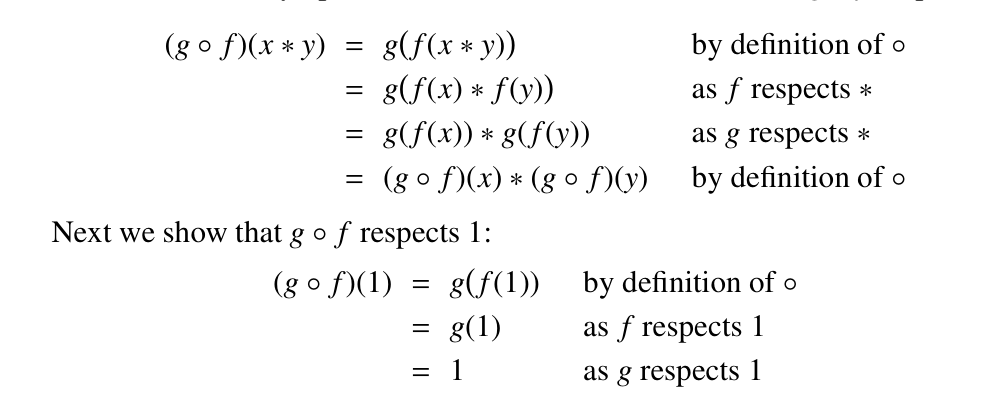
\includegraphics[width=0.9\textwidth]{imgs/13-01-monoid-homomorphism.png}
   \caption{$\circ$ for function composition,$\times$ for binary monoid
   operation}
\end{figure}
\begin{align}
    f =& 1\circ f &&\text{left unit}\\
    \times(1\circ f) =& \times(1) \circ \times(f) &&\text{left unit}\\
    \times(f) =& 1 \circ \times(f) &&\text{left unit}\\
    \times(f) =& \times(f) &&\text{left unit}\\
    f =& f\circ 1 &&\text{right unit}\\
    \times (f\circ 1) =& \times(f) \circ \times(1) &&\text{right unit}\\
    \times (f) =& \times(f) \circ 1 &&\text{right unit}\\
    \times (f) =& \times(f) &&\text{right unit}\\
    f\circ (g\circ h)=& (f\circ g) \circ h &&\text{associativity}\\
    \times(f\circ (g\circ h))=& \times(f\circ g) \circ \times(h) &&\text{associativity}\\
    \times(f\circ (g\circ h))(x)=& \times(f\circ g) \circ \times(h)(x) &&\text{associativity}\\
    \times(f\circ (g(h(x))))=& \times(f\circ g) \circ \times h(x) &&\text{associativity}\\
    \times(f(g(h(x))))=& \times(f\circ g) \circ \times h(x) &&\text{associativity}\\
\end{align}
\end{proofitem}
